\documentclass[10pt]{article}

% packages
\usepackage{wrapfig}
\usepackage{verbatim}
\usepackage{amsmath}
\usepackage{amssymb}
\usepackage{amsthm}
\usepackage{array}
\usepackage{xy}
\usepackage{geometry}
\usepackage{enumitem}
\setlist{nolistsep}


% page formatting
\pdfpagewidth 8.5in
\pdfpageheight 11in
\oddsidemargin -.25in
\textwidth 6.75in
\textheight 9in
\topmargin -1.75in
\headheight 112pt
 
\usepackage[pdftex]{graphicx}
\usepackage{asymptote}
\usepackage{fancyhdr}
 
\pagestyle{fancy}
\fancyhf{}

 
 
 

% Header with logo
\lhead{\includegraphics{EPHeaderleft.png}}
\rhead{\includegraphics{EPHeaderright.png}}
% Footer
\cfoot{Copyright $\copyright$ 2012-16\hskip0.044in -- \hskip0.044in {\scalebox{.354} {\includegraphics{EPFooter.png}}}} 


\linespread{1.15}
\begin{document}



\setlength{\abovedisplayskip}{-10.2pt}
\setlength{\belowdisplayskip}{6.8pt}
\setlength{\abovedisplayshortskip}{0pt}
\setlength{\belowdisplayshortskip}{0pt}


\centerline{\huge{2016 EP MC B Handouts}}


\clearpage

\centerline{\Large{Eat Pie Curriculum Pledge}} \vskip.1in

\centerline{\textbf{\noindent Please return by Monday, June 8, 2015.}}  \vskip0.33in

\noindent \emph{In order to maintain the intellectual integrity of the Eat Pie interns and instructors, I pledge that I will not share or distribute any classroom handouts, notes, materials, or problems sheets from $e\alpha\tau\cdot\pi ie$, with anybody. This includes friends, parents of friends, math team coaches, teachers, or other students at school who might ask for them.}

\vskip.5in
\centerline{\underline{\hskip6.5in}}\vskip.1in
\centerline{\underline{\hskip6.5in}}\vskip.1in
\centerline{\underline{\hskip6.5in}} \vskip0.1in
\centerline{\underline{\hskip6.5in}}\vskip.7in



Your signature: \underline{\hskip2in} \hskip1.8in Your name:\\ \\
\indent Signature of Agreeing Parent: \underline{\hskip2in}
\vskip.5in



\dotfill\\ \\ \\ 
\centerline{Congratulations! From now on, you will be under an honor code that you will not share any $e\alpha\tau\cdot\pi ie$}
\centerline{materials, problem sheets, or note handouts with anyone or the parties mentioned above.}
\\ \\
\centerline{If any parents, students, or math team teachers ask you to look at Eat Pie's materials, please direct them}
\centerline{to instructor.eatpie@gmail.com. Thank you for your cooperation.}
\\ \\ \\ \\ 
\centerline{\underline{\hskip2in}}
\centerline{The Eat Pie Team}


\vskip.7in

\clearpage

\centerline{\textbf{\Large{Pythagorean Theorem}}}

\vskip0.5in

\textbf{The Theorem}: If a right triangle has legs of length $a$ and $b$ and a hypotenuse of length $c$, then \fbox{$a^2+b^2=c^2$}
\vskip0.2in
\textbf{Pythagorean Triples}: When all three sides of a right triangle are integers. Some common ones:
\vskip0.1in
\begin{itemize}
\item 3-4-5
\item 5-12-13
\item 7-24-25
\item 8-15-17
\item 20-21-29
\item 28-45-53
\end{itemize}
\vskip0.2in

\textbf{When to use Pythagorean Theorem}
\vskip0.1in
\begin{itemize}
\item Whenever we have a right angle, consider it
\vskip0.05in
\begin{itemize}
\item Typically with rectangles and squares
\end{itemize}
\vskip0.05in
\item Almost every time we are asked for a length or a shortest distance
\vskip0.05in
\item Often when we need to find the area of a triangle
\end{itemize}
\vskip0.25in

\textbf{Problems!}
\vskip0.3in
\begin{itemize}

% 360
\item A diagonal of a rectangle is 41 inches, and the perimeter is 98 inches. What is the number of square inches in the area of the rectangle? (2000 National Sprint)
\vskip0.08in
\begin{itemize}
\setlength{\itemindent}{2em}
\item \emph{Solu.:} \hskip0.1in 
\end{itemize}
\vskip0.8 in

% 660
\item Isosceles triangle $BAD$ has side lengths of $61$ and $22$. What is the area of $\triangle BAD$?
\vskip0.08in
\begin{itemize}
\setlength{\itemindent}{2em}
\item \emph{Solu.:} \hskip0.1in 
\end{itemize}
\vskip0.8 in

% 70
\item Let $\triangle ABC$ be an equilateral triangle and $P$ a point on $\overline{BC}$. If $PB=50$ and $PC=30$, compute $PA$. (CMIMC 2016)
\vskip0.08in
\begin{itemize}
\setlength{\itemindent}{2em}
\item \emph{Solu.:} \hskip0.1in 
\end{itemize}
\vskip0.8 in

\clearpage

% 84
\item What is the area of a 13-14-15 triangle?
\vskip0.08in
\begin{itemize}
\setlength{\itemindent}{2em}
\item \emph{Solu.:} \hskip0.1in 
\end{itemize}
\vskip0.8 in

\end{itemize}

\textbf{With another dimension...}

\vskip0.3in

\begin{itemize}
% 10\sqrt{6}
\item A rectangular prism measures $10$-inches by $20$-inches by $10$-inches. What is the length, in inches, of the diagonal connecting point $A$ and point $B$? Express your answer in simplest radical form. (2009 State Target)

\centerline{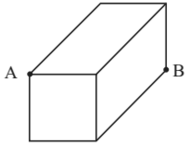
\includegraphics{20092.PNG}}
\vskip0.08in
\begin{itemize}
\setlength{\itemindent}{2em}
\item \emph{Solu.:} \hskip0.1in 
\end{itemize}
\vskip0.8 in

% 96
\item A right pyramid has a square base that measures 10 cm on each side. Its peak is 12 cm above the center of its base. What is the sum of the lengths of the pyramid's eight edges? Express your answer as a decimal to the nearest whole number. (2008 State Target)
\vskip0.08in
\begin{itemize}
\setlength{\itemindent}{2em}
\item \emph{Solu.:} \hskip0.1in 
\end{itemize}
\vskip0.8 in

% 100\sqrt{5}
\item The Yerts live on planet Yetterbia, which is shaped like a cube of side length 100 miles. Pert the Yert is on one of the corners of the planet. Bert the Yert is standing as far away from Pert as possible. What is the shortest distance, in miles, that Pert can walk on the surface of the planet to get to Bert?
\vskip0.08in
\begin{itemize}
\setlength{\itemindent}{2em}
\item \emph{Solu.:} \hskip0.1in 
\end{itemize}
\vskip0.8 in


\end{itemize}

\clearpage

\centerline{\textbf{\Large{Pythagorean Practice}}}

\vskip0.5in
\begin{enumerate}

% 10, 17, 2\sqrt{13}, \sqrt{37}/2, 
\item Find the hypotenuse of the right triangle with the leg lengths given in each of the following:

\begin{itemize}
\item 6, 8
\item 8, 15
\item 4, 6
\item 0.5, 3
\item 180, 189
\end{itemize}

\vskip0.26in

% 71
\item Suppose a very poorly designed bridge 10,000 feet long expands in length by one foot on a warm summer day. Because the side supports do not move, the middle of the bridge sags downward, making two straight, congruent line segments as shown. How many feet below the original bridge's height is the middle (A) of the lengthened bridge? Express your answer to the nearest whole number. (2007 State Target)

\centerline{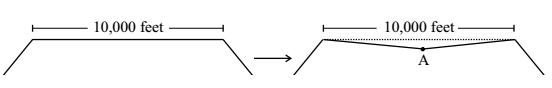
\includegraphics{20072.PNG}}

\vskip0.16in

% 225
\item Sohan takes a walk starting at his house. He heads east but after walking for 135 meters in that direction, he runs into Sam. The two of them decide to go to the nearest froyo shop which is 180 meters to the south. How far away from home is Sohan when he gets there?

\vskip0.26in

% 420
\item In $\bigtriangleup ABC$, $AB=BC=29$, and $AC=42$. What is the area of $\bigtriangleup ABC$? (2015 AMC 8)
\vskip0.26in


% 13
\item Rectangle $ABCD$ and right triangle $DCE$ have the same area. They are joined to form a trapezoid, as shown. What is $DE$? (2014 AMC 8)
\vskip0.05in
\begin{center}
\begin{asy}
import olympiad;
size(150);
defaultpen(linewidth(0.8));
pair A=(0,5),B=origin,C=(6,0),D=(6,5),E=(18,0);
draw(A--B--E--D--cycle^^C--D);
draw(rightanglemark(D,C,E,30));
label("$A$",A,NW);
label("$B$",B,SW);
label("$C$",C,S);
label("$D$",D,N);
label("$E$",E,S);
label("$5$",A/2,W);
label("$6$",(A+D)/2,N);
\end{asy}
\end{center}
\vskip0.26in

% 5.29
\item A triangle has a side of length 6 cm, a side of length 8 cm, and a right angle. What is the shortest possible length of the remaining side of the triangle? Express your answer as a decimal to the nearest hundredth. (2006 State Target)

\vskip0.26in


% 2\sqrt{41}
\item The asteroid Daedalus is shaped like a rectangular prism measuring 5 miles by 5 miles by 8 miles. If Joshua and Yashi are standing at opposite vertices of the asteroid, what is the shortest distance Yashi could walk along the surface of the asteroid to get to Joshua?

\end{enumerate}

\clearpage


\centerline{\textbf{\Large{Special Right Triangles}}}

\vskip0.5in

Right triangles are always useful, but certain right triangles are especially useful.

\vskip0.3in
\textbf{Diagrams and Properties}
\vskip1.4in
\textbf{Quick Flowchart}
\vskip0.1in
\begin{itemize}
\item Notice an angle like 30, 45, 60, 120, 135, or 150
\vskip0.05in
\item If there's no obvious right angle, drop an altitude
\vskip0.05in
\item Once you have the right triangle, define variables if necessary and solve
\end{itemize}
\vskip0.25in

\textbf{Problems!}
\vskip0.3in
\begin{itemize}


% 5+4\sqrt{3}
\item An equilateral triangle has two vertices at $(0,5)$ and $(8,5)$. If the third vertex is in the first quadrant, what is its y-coordinate? Express your answer in simplest radical form. (2010 Chapter Sprint)
\vskip0.08in
\begin{itemize}
\setlength{\itemindent}{2em}
\item \emph{Solu.:} \hskip0.1in 
\end{itemize}
\vskip0.8 in

% 6\sqrt{7}
\item A 30-60-90 triangle is drawn on the exterior of an equilateral triangle so that the hypotenuse of the right triangle is one side of the equilateral triangle. If the shorter leg of the right triangle is 6 units, what is the distance between the two vertices that the triangles do not have in common? Express your answer in simplest radical form. (2008 National Target)

\centerline{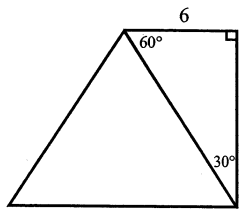
\includegraphics[scale=0.5]{20083.PNG}}
\vskip0.08in
\begin{itemize}
\setlength{\itemindent}{2em}
\item \emph{Solu.:} \hskip0.1in 
\end{itemize}
\vskip0.8 in


% 5.5 
\item Alice and Bob live $10$ miles apart. One day Alice looks due north from her house and sees an airplane. At the same time Bob looks due west from his house and sees the same airplane. The angle of elevation of the airplane is $30^\circ$ from Alice's position and $60^\circ$ from Bob's position. Which of the following is closest to the airplane's altitude, in miles? (2016 AMC 12B)
\vskip0.08in
\begin{itemize}
\setlength{\itemindent}{2em}
\item \emph{Solu.:} \hskip0.1in 
\end{itemize}
\vskip0.8 in


% 12\sqrt{3}
\item Six circles of radius 1 unit are drawn tangent to the sides of a regular hexagon. Each circle is also tangent to two other circles as shown in the drawing. What is the perimeter of the hexagon? Express your answer in simplest radical form. (2012 Chapter Sprint)

\centerline{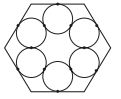
\includegraphics{2012HexSprint.PNG}}
\vskip0.08in
\begin{itemize}
\setlength{\itemindent}{2em}
\item \emph{Solu.:} \hskip0.1in 
\end{itemize}
\vskip0.8 in



\end{itemize}

\clearpage

\centerline{\textbf{\Large{Special Right Tri-gons}}}

\vskip0.5in
\begin{enumerate}


% \sqrt{3}
\item An equilateral triangle, with sides of length 2 units has a circular arc centered at $B$, inscribed as shown. What is the length of a segment drawn parallel to side $AC$ with endpoint $D$ and $E$? Express your answer in simplest radical form. (2014 Chapter Sprint)

\centerline{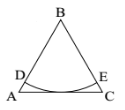
\includegraphics{201423.png}}

\vskip0.26in

% 32
\item The shaded region consists of 16 congruent squares. If $PQ=6$ cm, what is the area of the entire shaded region? (2005 State Sprint)

\centerline{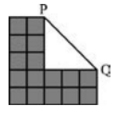
\includegraphics{200527.PNG}}

\vskip0.26in


% 30+10\sqrt{3}
\item Maanasi is on a trip to climb Mount Meringue. From her starting point, the angle of elevation to the top of the mountain is $45^\circ$. After walking 20 meters toward the mountain, the angle of elevation is now $60^\circ$. In simplest radical form, what is the height of the mountain?

\vskip0.26in

% 6\sqrt{3}+18
\item Two angles of a triangle measure 30 and 45 degrees. If the side of the triangle opposite the 30-degree angle measures $6\sqrt{2}$ units, what is the sum of the lengths of the two remaining sides? Express your answer as a decimal to the nearest tenth. (2009 State Team)
\vskip0.26in




% 10\sqrt{3}
\item In pentagon $ABCDE$, $\angle E$ and $\angle C$ are right angles and $m\angle D=120^\circ$. If $AB=12$, $AE=BC=18$, and $ED=DC$, what is $ED$? Express your answer in simplest radical form. (2015 State Sprint)

\vskip0.26in

% \sqrt{3}
\item A circle is inscribed in a rhombus with sides of length 4 cm. If the two acute angles in the rhombus each measure $60^\circ$, what is the length of the circle's radius? Express your answer in simplest radical form. (2012 Chapter Sprint)

\centerline{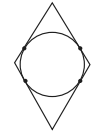
\includegraphics{2012RhombusSprint.PNG}}

\vskip0.26in

% 45
\item Coplanar points $A$, $B$, $C$, $D$, and $E$ are arranged such that $A$, $B$, and $C$ are collinear with $B$ between $A$ and $C$, triangle $ABD$ is equilateral, triangle $BEC$ is isosceles with congruent legs $\overline{BE}$ and $\overline{EC}$ , and points $D$ and $E$ are on the same side of line $AC$. The measure of $\angle EBC$ is 30 degrees. the areas of triangles $ABD$ and $BEC$ are equal. What is the number of degrees in the measure of $\angle BDE$? (2005 State Team)

\centerline{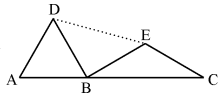
\includegraphics{20056.png}}

\vskip0.26in






\end{enumerate}

\clearpage

\centerline{\textbf{\Large{Introduction to Probability}}}


\vskip 0.4in

The probability of event $a$ happening is the $\#$ of favorable outcomes over the total outcomes: $P(a)=\frac{a}{total}$.

\

\

\textbf{Basic Probability}

\textit{Example:}
\begin{itemize}
\setlength{\itemindent}{2em}

\item \textbf{How many ways are there to roll a 7 with two standard dice?}
\begin{itemize}
\item \textit{Solution:} There are 6 ways to roll a 7, out of 36 total ways to roll.  The probability is $\boxed{\frac{1}{6}}$.
\end{itemize}
\end{itemize}

\vskip0.15in

\textit{Example 2:}
\begin{itemize}
\setlength{\itemindent}{2em}

\item \textbf{A $4\times4\times4$ cube is painted then cut into 64 identical cubes.  Find the probability that if a random cube is selected it will have exactly 2 faces painted.}
\begin{itemize}
\item \textit{Solution:} The cubes with 2 faces painted are the cubes on the edges of the original cube.  There are 12 edges $\times$ 2 per edge = 24 cubes.  The probability is $\frac{24}{64}=\boxed{\frac{3}{8}}$
\end{itemize}
\end{itemize}

\vskip1in

\textbf{Complementary Probability}

Used in the scenario in which counting the cases that \emph{don't work} is easier:  $P(a) = 1-P($not $a)$.

\textit{Example:}
\begin{itemize}
\setlength{\itemindent}{2em}

\item \textbf{What is the probability that when a coin is flipped five times, there will be at least one head?}
\begin{itemize}
\item \textit{Solution:} $P($one head or more$)$ = $1-P($no heads$)$.  The probability that there will be no heads is $\frac{1}{32}$.  The probability that there will be at least one head is $1-\frac{1}{32}=\boxed{\frac{31}{32}}$.
\end{itemize}
\end{itemize}

\vskip1in

\textbf{Conditional Probability}

\hskip.5in The probability of an event $a$ while another event $b$ is already guaranteed to happen.

\hskip.5in Probability of event $a$ with condition $b$ (given $b$): $P(a)=\frac{P(a \& b)}{P(b)}$.

\
\textit{Example:}
\begin{itemize}
\setlength{\itemindent}{2em}

\item \textbf{A coin is flipped 3 times.  If the first flip came up heads, what is the probability that all three flips will be heads?}
\begin{itemize}
\item \textit{Solution:} There is only one way to flip heads all three times.  Since the first flip is heads, then there are only 4 ways for the other two flips.  The probability is $\boxed{\frac{1}{4}}$.
\end{itemize}
\end{itemize}

\vskip0.15in



    
\clearpage

\centerline{\textbf{\Large{Probability: General and Complementary}}} \vskip0.1in
\vskip0.33in

\begin{enumerate}

% 
% Answer: 2/3
\item One student in a class of boys and girls is to be chosen to represent the class. Each student is equally likely to be chosen and the probability that a boy is chosen is 2/3 of the probability that a girl is chosen. Find the ratio of the number of boys to the total number of boys and girls. \emph{(AHSME)}

\vskip0.26in




%
% Answer: 2/3
\item Allie and Barry play a game in which they take turns flipping a fair coin until one of them flips heads. The winner is the first person to flip a head. If Allie goes first, find the probability that she wins.

\vskip0.26in




% 
% Answer: 15/16
\item Four numbers are randomly selected, with replacement, from the set of integers 1 through 100 
inclusive. What is the probability that the product of the four numbers selected will be even? 

\vskip0.26in

% 9/20
\item Bag $A$ contains 3 white and 2 red balls. Bag $B$ contains 6 white and 3 red balls. One of the two bags will be chosen at random, and then two balls will be drawn from that bag at random without replacement. What is the probability that the two balls drawn will be the same color? Express your answer as a common fraction. (2010 State Sprint)
\vskip0.26in

% 969
\item My three-digit code is 023. Reckha can't choose a code that is the same as mine in two or more of the three digit-positions, nor that is the same as mine except for switching the positions of two digits (so 320 and 203, for example, are forbidden, but 302 is fine). Reckha can otherwise choose any three-digit code where each digit is in the set $\{0, 1, 2, 3, 4, 5, 6, 7, 8, 9\}$. How many codes are available for Reckha? (2006 State Target)

\vskip0.26in

% 
% Answer: 1/10,000,000
\item Let $S$ be the set of all 15-digit positive integers. An integer is chosen at random from $S$. Find the 
probability that the integer is a palindrome. \emph{(NYSML)}

\vskip0.26in



% 
% Answer: 7/30
\item The ten letters of the word MATHCOUNTS are written on cards, one letter per card, and placed in a basket. When two cards are picked at random without replacement, what is probability that the first card chosen has a vowel on it and the second card chosen has a consonant? Express your answer as a common fraction. \emph{(MATHCOUNTS)} 

\vskip0.26in




%
% Answer: .504
\item A typical ID number in a college class consists of a four-digit number, such as 0119. When an ID number is randomly selected, what is the probability that no two digits are the same? Express your answer as a decimal to the nearest thousandths. \emph{(MATHCOUNTS)}

\vskip0.26in



%
% Answer: 7/8
\item Three integers are picked at random from the set $\{1,2,3,\dots,99,100\}$.  Find the probability that their product is even.

\vskip0.26in



%
% Answer: 844/969
\item A bag of 20 marbles has five red, five green, five blue, and five yellow marbles. Four marbles are randomly selected (without replacement). What is the probability that two or more marbles are the same color? \emph{(Mu Alpha Theta)}
\vskip0.26in

% 5/32
\item The four faces of a fair tetrahedral die are numbered one, two, three and four. Each time the die is rolled, three numbers are visible. If the die is rolled three times, what is the probability that the sum of all nine of the numbers showing is $21$? Express your answer as a common fraction. (2011 National Target)

\vskip0.26in

% 7
\item How many of the divisors of $8!$ are larger than $7!$ ? (2002 National Sprint)

\vskip0.26in

\end{enumerate}

\clearpage

\centerline{\Large{\underline{Mock MATHCOUNTS Target}}}
\vskip 0.7cm

\begin{enumerate}

% 2\sqrt{13}
\item Side $AB$ of regular hexagon $ABCDEF$ is extended past $B$ to point $X$ such that $AX=3AB$. Given that each side of the hexagon is 2 units long, what is the length of segment $FX$? Express your answer in simplest radical form. (2010 National Sprint)
\vskip 7.5cm

\hskip 12cm
\fbox{
	\begin{minipage}{1in}
		\hfill \vspace{0.6in}
	\end{minipage}
	}
	\vskip0.1in
\

\

\

% 13
\item Rectangle $ABCD$ is shown with $AB=6$ units and $AD=5$ units. If $AC$ is extended to point $E$ such that $\overline{AC}$ is congruent to $\overline{CE}$, what is the length of $\overline{DE}$? (2016 State Sprint)

\centerline{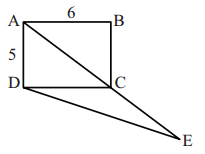
\includegraphics{201618.png}}

\vskip0.6in
\hskip 12cm
\fbox{
	\begin{minipage}{1in}
		\hfill \vspace{0.6in}
	\end{minipage}
	}
	\vskip0.1in

\end{enumerate}

\clearpage

\centerline{\textbf{\Large{Similarity}}} \vskip0.1in
\centerline{\textit{...all the same to me}}
\vskip0.33in

\begin{itemize}


\renewcommand{\labelitemi}{$\bullet$ \hskip0.04in}
\renewcommand{\labelitemii}{$\cdot$}
\renewcommand{\labelitemiii}{--}
\renewcommand{\labelitemiv}{$\ast$}

\item \textbf{Tipoffs}
\vskip0.17in
\begin{itemize}
\item Equal angles in separate figures typically suggest similarity
\item Parallel lines, vertical angles, shared angles, and occasionally right angles give equal angles
\begin{itemize}
\item Rectangles and trapezoids are the most common carriers of these
\end{itemize}
\item If you're stuck on a (geometry) problem, at least briefly consider the possibility of similarity 

\end{itemize}
\vskip0.17in
\item \textbf{Takeaways}
\vskip0.17in
\begin{itemize}
\item Always identify which sides correspond to which in a similarity
\item Suppose that the ratio of similarity between two figures is $k$
\begin{itemize}
\item The ratio of \emph{any} corresponding lengths is $k$
\item The ratio of areas is $k^2$ and the ratio of volumes are $k^3$
\end{itemize}
\end{itemize}

\vskip0.17in
\item \textbf{Setups}

\vskip0.3in

\begin{center}

\includegraphics{Similarity1.PNG}
%
%
\begin{comment}
\begin{asy}
import graph; size(12cm); 
real labelscalefactor = 0.5; /* changes label-to-point distance */
pen dps = linewidth(0.7) + fontsize(10); defaultpen(dps); /* default pen style */ 
pen dotstyle = black; /* point style */ 
real xmin = -1.5348513784428954, xmax = 8.219393844124252, ymin = -0.15273649023160163, ymax = 4.571710978437879;  /* image dimensions */
pen qqwuqq = rgb(0.,0.39215686274509803,0.); 

draw(arc((1.109729729729731,3.52),0.5089171420469816,-35.433314010285585,0.)--(1.109729729729731,3.52)--cycle, qqwuqq); 
draw(arc((4.7918918918918925,0.9),0.5089171420469816,144.56668598971444,180.)--(4.7918918918918925,0.9)--cycle, qqwuqq); 
draw(arc((2.454347826086956,0.9),0.2544585710234908,0.,78.92979742206059)--(2.454347826086956,0.9)--cycle, qqwuqq); 
draw(arc((2.9669565217391307,3.52),0.2544585710234908,180.,258.92979742206063)--(2.9669565217391307,3.52)--cycle, qqwuqq); 
 /* draw figures */
draw((xmin, 0.*xmin + 0.9)--(xmax, 0.*xmax + 0.9)); /* line */
draw((xmin, 0.*xmin + 3.52)--(xmax, 0.*xmax + 3.52)); /* line */
draw((xmin, -0.7115384615384616*xmin + 4.309615384615386)--(xmax, -0.7115384615384616*xmax + 4.309615384615386)); /* line */
draw((xmin, 5.111111111111106*xmin-11.644444444444431)--(xmax, 5.111111111111106*xmax-11.644444444444431)); /* line */
draw(arc((1.109729729729731,3.52),0.5089171420469816,-35.433314010285585,0.), qqwuqq); 
draw(arc((1.109729729729731,3.52),0.4665073802097331,-35.433314010285585,0.), qqwuqq); 
draw(arc((4.7918918918918925,0.9),0.5089171420469816,144.56668598971444,180.), qqwuqq); 
draw(arc((4.7918918918918925,0.9),0.4665073802097331,144.56668598971444,180.), qqwuqq); 
 /* dots and labels */
dot((-1.24,0.9),dotstyle); 
dot((7.78,0.9),dotstyle); 
dot((1.08,3.52),dotstyle); 
dot((2.74,2.36),dotstyle); 
dot((3.78,1.62),dotstyle); 
dot((2.56,1.44),dotstyle); 
dot((4.7918918918918925,0.9),linewidth(3.pt) + dotstyle); 
dot((2.454347826086956,0.9),linewidth(3.pt) + dotstyle); 
dot((2.9669565217391307,3.52),linewidth(3.pt) + dotstyle); 
clip((xmin,ymin)--(xmin,ymax)--(xmax,ymax)--(xmax,ymin)--cycle); 
\end{asy}
\end{comment}
%
\hskip0.2in
%
\begin{comment}
\begin{asy}
import graph; size(20.cm); 
real labelscalefactor = 0.5; /* changes label-to-point distance */
pen dps = linewidth(0.7) + fontsize(10); defaultpen(dps); /* default pen style */ 
pen dotstyle = black; /* point style */ 
real xmin = -5, xmax = 8, ymin = -2, ymax = -1;  /* image dimensions */
pen qqwuqq = rgb(0.,0.39215686274509803,0.); 

draw(arc((2.661268598277212,2.472748629600626),0.6,112.94893728092329,178.42525493424682)--(2.661268598277212,2.472748629600626)--cycle, qqwuqq); 
draw(arc((5.556593265465936,2.393152075176194),0.6,112.94893728092329,178.42525493424682)--(5.556593265465936,2.393152075176194)--cycle, qqwuqq); 
draw(arc((1.763992273019961,4.59184803605924),0.6,-146.1887999282518,-67.05106271907671)--(1.763992273019961,4.59184803605924)--cycle, qqwuqq); 
draw(arc((3.9934037347070186,6.0849401159047005),0.6,-146.1887999282518,-67.05106271907673)--(3.9934037347070186,6.0849401159047005)--cycle, qqwuqq); 
 /* draw figures */
draw((xmin, -2.361702127659574*xmin + 8.75787234042553)--(xmax, -2.361702127659574*xmax + 8.75787234042553)); /* line */
draw((xmin, -2.361702127659574*xmin + 15.516170212765957)--(xmax, -2.361702127659574*xmax + 15.516170212765957)); /* line */
draw((-1.24,2.58)--(xmax, 0.6697247706422018*xmax + 3.41045871559633)); /* ray */
draw((-1.24,2.58)--(xmax, -0.027491408934707928*xmax + 2.545910652920962)); /* ray */
draw(arc((2.661268598277212,2.472748629600626),0.6,112.94893728092329,178.42525493424682), qqwuqq); 
draw(arc((2.661268598277212,2.472748629600626),0.5,112.94893728092329,178.42525493424682), qqwuqq); 
draw(arc((2.661268598277212,2.472748629600626),0.4,112.94893728092329,178.42525493424682), qqwuqq); 
draw(arc((5.556593265465936,2.393152075176194),0.6,112.94893728092329,178.42525493424682), qqwuqq); 
draw(arc((5.556593265465936,2.393152075176194),0.5,112.94893728092329,178.42525493424682), qqwuqq); 
draw(arc((5.556593265465936,2.393152075176194),0.4,112.94893728092329,178.42525493424682), qqwuqq);
\end{asy}
\end{comment}
%
%
\includegraphics{Similarity2.PNG}

\end{center}

\vskip0.5in



\item \textbf{Problems!}
\vskip0.3in

\begin{itemize}

% 3
\item In rectangle $ABCD$, $BC=2AB$. Points $O$ and $M$ are the midpoints of $\overline{AD}$ and $\overline{BC}$, respectively. Point $P$ bisects $\overline{AO}$. Let $N$ be the intersection of $OB$ and $PM$. If $OB=6\sqrt{2}$ units, what is the area of $\triangle NOP$? (2013 MC State Target)

\vskip0.08in
\begin{itemize}
\setlength{\itemindent}{2em}
\item \emph{Solu.:} \hskip0.1in 
\end{itemize}
\vskip0.8 in

\clearpage

% 72
\item Trapezoid $ABCD$ has base $AB=20$ units and base $CD=30$ units. Diagonals $AC$ and $BD$ intersect at $X$. If the area of trapezoid $ABCD$ is 300 square units, what is the area of triangle $BXC$? (2010 State Target)

\vskip0.08in
\begin{itemize}
\setlength{\itemindent}{2em}
\item \emph{Solu.:} \hskip0.1in 
\end{itemize}
\vskip0.8 in








% 1225/72
\item Rectangle $ABCD$ is inscribed in triangle $EFG$ such that side $AD$ of the rectangle is on side $EG$ of the triangle, as shown. The triangle's altitude from $F$ to side $EG$ is 7 inches, and $EG=10$ inches. The length of segment $AB$ is equal to half the length of the segment $AD$. What is the area of rectangle $ABCD$? Express your answer as a common fraction. (2007 National Team)

\centerline{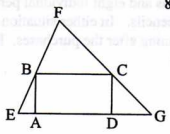
\includegraphics{2007NatTeam.PNG}}

\vskip0.08in
\begin{itemize}
\setlength{\itemindent}{2em}
\item \emph{Solu.:} \hskip0.1in 
\end{itemize}
\vskip0.8 in














% 25pi
\item When the diameter of a pizza increases by 2 inches, the area increases by $44\%$. What was the area, in square inches, of the original pizza? Express your answer in terms of $\pi$. (2011 State Sprint)

\vskip0.08in
\begin{itemize}
\setlength{\itemindent}{2em}
\item \emph{Solu.:} \hskip0.1in 
\end{itemize}
\vskip0.8 in




% 32
\item A right square pyramid with base edges of length $8\sqrt{2}$ units each and slant edges of length 10 units each is cut by a plane that is parallel to its base and 3 units above its base. What is the volume, in cubic units, of the new pyramid that is cut off by this plane? (2009 National Target)

\vskip0.08in
\begin{itemize}
\setlength{\itemindent}{2em}
\item \emph{Solu.:} \hskip0.1in 
\end{itemize}
\vskip0.8 in







\end{itemize}

\end{itemize}

\clearpage

\centerline{\textbf{\Large{Similarity Problems}}} 
\vskip0.5in

\begin{enumerate}

% 81
\item In trapezoid $ABCD$ segments $AB$ and $CD$ are parallel. Point $P$ is the intersection of diagonals $AC$ and $BD$. The area of $\triangle PAB$ is 16 square units, and the area of $\triangle PCD$ is 25 square units. What is the area of trapezoid $ABCD$? (2012 State Sprint)

\vskip0.26in

% 174
\item The surface area of sphere $A$ is $96\%$ more than the surface area of sphere $B$. The volume of sphere $A$ is $r\%$ more than the volume of sphere $B$. What is the value of $r$? Express your answer to the nearest whole number. (2001 Nats Target)

\vskip0.26in

% 98
\item In a trapezoid $ABCD$ with $AB$ parallel to $CD$, the diagonals $AC$ and $BD$ intersect at $E$. If the area of triangle $ABE$ is 50 square units, and the area of triangle $ADE$ is 20 square units, what is the area of trapezoid $ABCD$? (2009 Nats Sprint)




\vskip0.26in

% 4/21
\item In rectangle $ABCD$, points $E$ and $F$ lie on segments $AB$ and $CD$, respectively, such that $AE=\frac{AB}{3}$ and $CF=\frac{CD}{2}$. Segment $BD$ intersects segment $EF$ at $P$. What fraction of the area of rectangle $ABCD$ lies in triangle $EBP$? Express your answer as a common fraction. (2010 State Sprint)

\vskip0.26in

% 72/13
\item  In the figure below, a 3-inch by 3-inch square adjoins a 10-inch by 10-inch square. What is the area of the region $CDFE$? Express your answer in square inches as a common fraction. (2009 State Target)

\centerline{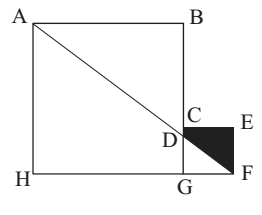
\includegraphics{20097.PNG}}

\vskip0.13in

% 19/37
\item A right circular cone is sliced into four pieces by planes parallel to its base, as shown in the figure. All of these pieces have the same height. What is the ratio of the volume of the second-largest piece to the volume of the largest piece? Express your answer as a common fraction. (2011 State Sprint)

\centerline{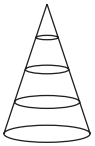
\includegraphics{2011Sprint.PNG}}

\vskip0.26in


% \sqrt{7}
\item In rectangle $ABCD$, $AB=6$ units, the measure of $\angle DBC$ is $30^{\circ}$, $M$ is the midpoint of segment $AD$ and segments $CM$ and $BD$ intersect at $K$. What is the length of segment $MK$? Express your answer in simplest radical form. (2012 MC State Sprint)

\vskip0.26in




% 42
\item In square units, what is the largest possible area a rectangle inscribed in a 10-17-21 triangle can have? (2013 State Sprint)

\end{enumerate}

\clearpage

\centerline{\textbf{\Large{The Division Theorem:}}} \vskip0.1in
\centerline{\textbf{\textsc{AKA} ``The Remainder Structure of Integers"}}
\vskip0.33in

\begin{itemize}


\renewcommand{\labelitemi}{$\bullet$ \hskip0.04in}
\renewcommand{\labelitemii}{$\cdot$}
\renewcommand{\labelitemiii}{$\diamond$}
\renewcommand{\labelitemiv}{$\ast$}

\item \textbf{Division Theorem:} \hskip0.1in There is exactly one way to express each integer $x$ in the form \hskip0.03in $x = pq + r$,
where $p$, $q$, and $r$ are integers, such that $p$ is the divisor, $q$ is the quotient, and $r$ is the remainder, for which $0 \le r < q$. (In other words, division works).
\vskip0.17in

\begin{itemize} 
\item \emph{Example:}  $100 = 14\cdot 7 + 2$, or 100 days can be divided into 14 weeks with 2 days left over.
\end{itemize}
\vskip0.65in





\item \textbf{Problem 1:} \hskip0.1in  If the last day of 1996 was a Monday, what day of the week is February 23, 1997?
\vskip0.15in
\begin{itemize}
\item \emph{Solution:} \hskip0.1in Since December 31, 1996, is a Monday, we are trying to find the day of the week that is 31 + 23 days after a Monday.  So: 31 + 23 = 54, and $54 = 7\cdot 7 + 5$.
Therefore, 5 days after Monday is Saturday, so Feb. 23, 1997 is a Saturday.

\vskip0.32in

\centerline{\emph{But There's Got To Be a Better Way!}}
\vskip0.27in 

\centerline{Another way to do this problem is to just drop the multiples of 7} 
\centerline{under 31 and 23, and we find that there are 3 and 2 extra days respectively.}
\end{itemize}
\end{itemize}

\begin{align*}
31=4\cdot 7+3 \\
23=3\cdot 7+2
\end{align*}

\centerline{Now, we can just \textbf{\underline{add remainders}} to get 3 + 2 = 5 days more than an integral number} 
\centerline{of weeks.  So 5 days after Monday is Saturday, which makes Feb. 23, 1997, a Saturday.}
\vskip0.6 in





\begin{itemize}


\renewcommand{\labelitemi}{$\bullet$ \hskip0.04in}
\renewcommand{\labelitemii}{$\cdot$}
\renewcommand{\labelitemiii}{$\diamond$}
\renewcommand{\labelitemiv}{$\ast$}


\item \textbf{Problem 2:} \hskip0.1in  The first day of the twenty-first century was January 1, 2001, which was a Monday.  What day of the week will be the first day of the twenty-second century?
\vskip0.15in

\begin{itemize}
\item \emph{Solution:} \hskip0.1in The longer solution is to recognize that $365\cdot 100 + 24 = 36524$, where the extra 24 represents the extra days due to the leap years (contrary to what you might think, 2100 is not a leap year). \\

\centerline{$36524 = 5217\cdot 7 + 5$, so we now have found out that a century} 
\centerline{can be divided into 5217 weeks with 5 days left over.} 
	
\vskip0.15in \centerline{Therefore, 5 days after a Monday is Saturday, so Jan. 1, 2101, is a Saturday.}

\vskip0.32in

\centerline{\emph{But There's Got To Be a Better Way!}}
\vskip0.27in 

\centerline{The much quicker way to do this problem is to just drop the multiples} 
\centerline{of 7 under 365, and we find: $365 = 52\cdot 7 + 1$.} 

\vskip0.15in
\centerline{Therefore, one hundred years will give us 5200 weeks with 100 extra days, plus} 
\centerline{an additional 24 days to account for the leap years.  Now, we can forget about}
\centerline{the 5200 weeks and just consider the 124 extra days.}

\vskip0.15in
\centerline{$124 = 17\cdot 7 + 5,$}

\vskip0.15in \centerline{so there are 5 extra days after the 17 additional weeks.  Therefore, we} 
\centerline{find much more quickly that Saturday is the first day of year 2101.} 

\vskip0.32in

\centerline{\emph{But There's Got To Be an Even Better Way?!}}
\vskip0.27in 

 
\centerline{We can even further quicken this process by recognizing that $100 = 14\cdot 7 + 2$.  So} 
\centerline{over $14\cdot 7 = 98$ years, the single extra day in every year will be grouped into 98 days} 
\centerline{or 14 extra weeks.  Therefore, now we only need to consider the 2 extra days left,}
\centerline{plus the 24 extra days from the leap years.}
\vskip0.15in
\centerline{$2 + 24 = 26 = 3\cdot 7 + 5$.}

\vskip0.35in
\centerline{\emph{Summary:}} 
\vskip0.05in

\centerline{Method 1:  $100\cdot 365 + 24 = 36524 = 5217 + 5.$}
\centerline{Method 2:  $100\cdot 1 + 24 = 124 = 17\cdot 7 + 5.$}
\centerline{Method 3:  $2\cdot 1 + 24 = 26 = 3\cdot 7 + 5$}

\vskip0.15in
\centerline{Basically, by Method 3, we \textbf{\underline{multiplied the remainders}} 2 and 1, the respective}
\centerline{remainders when 100 and 365 are divided by 7.}
\end{itemize}




\vskip0.7in
\item \textbf{Problem 3:} \hskip0.1in  Find the remainder when $23^5$ is divided by 7.
\vskip0.15in

\begin{itemize}
\item \emph{Solution:} \hskip0.1in Since exponentiation is really just quick multiplication, we can apply our ``multiplying remainders" rule to this problem. \\

\centerline{$23^5 = 23\cdot 23\cdot 23\cdot 23\cdot 23$, which will have the same remainder as $2\cdot 2 \cdot 2\cdot 2\cdot 2 = 2^5$.} 

\vskip0.15in
\centerline{Therefore, we could have replaced 23 with 2 in our computations (Do you see why?)} 
\centerline{So now we just need to compute $2^5 = 32$, and $32 = 4\cdot 7 + 4$.  Therefore, $23^5$ leaves }
\centerline{a remainder of 4 when divided by 7.   That was easy!!}
\end{itemize}
\end{itemize}

\clearpage

\centerline{\textbf{\Large{Modular Arithmetic}}}
\vskip0.33in

Modular arithmetic, also called mods, is a branch of mathematics used to solve for remainders when an integer is divided by another integer. In other words, it's a sleeker, more compact version of the division theorem.
\vskip0.17in


\indent \indent  \indent $-$ \emph{Definition:}  $m\equiv n \bmod{p}$ is equivalent to $\frac{m-n}{p}\in N$. In other words, $m-n$ is a multiple of $p$. \\

\vskip-0.18in \hskip1.28in For example: $53\equiv 3\bmod{5}$. Note that the symbol $``\equiv"$ is used, not $``="$. \\ \vskip-0.18in \hskip1.28in Also, note that 5 is what we call our \textbf{modulus}.
\\ \vskip-0.18in \hskip1.28in
In terms of the Division Theorem, if $x=pq+r$, then $x\equiv r \bmod p$.


\vskip0.42in

\textbf{Why we care}: Mods  have their own system of arithmetic (hence, modular arithmetic)
\vskip0.05in
\begin{itemize}
\item $a+b\pmod{n}\equiv a\pmod{n}+b\pmod{n}$
\vskip0.05in
\item $a\times b\pmod{n}\equiv a\pmod{n}\times b\pmod{n}$

\end{itemize}

\vskip.2in

\begin{itemize}


\renewcommand{\labelitemi}{$\bullet$ \hskip0.04in}
\renewcommand{\labelitemii}{$\cdot$}
\renewcommand{\labelitemiii}{$\diamond$}
\renewcommand{\labelitemiv}{$\ast$}


\item \textbf{Find 109 mod 9}. 
\vskip0.08in
\begin{itemize} 
\item We start by finding the smallest multiple of 9 less than 109.  We know 90 is a multiple of 9, so we add 18, which is another multiple of 9, to get 108, another multiple of 9. Thus, $109 \equiv 109-108\equiv 1\bmod{9}$.
\end{itemize}


\vskip0.2in




\item \textbf{Find $-$2 mod 8.} 

\vskip0.08in
\begin{itemize}
\item This problem may look a bit strange at first, but thinking outside the box would definitely help. Let us subtract a negative multiple of 8:  $-2 \equiv -2-(-8) \equiv 6 \bmod{8}$.  Now we see that $-2\equiv 6\bmod{8}$.
\end{itemize}


\vskip0.2in


\item \textbf{Find the last digit of 8$\times$6$\times$7$\times$2$\times$13$\times$19.} 

\vskip0.08in
\begin{itemize}
\item The last digit of an integer is the remainder when the integer is divided by 10.  Let's rewrite each of the integers in mod 10.   This still looks rather messy, so we simplify by multiplying out the negatives.  Observing the problem above, we discover that
 $8\times 6\times 7\times 2\times 3\times 9 \equiv (-2)\times(-4)\times (-3) \times 2\times 3\times (-1) \equiv 8\times 9\times 2 \equiv 4 \bmod{10}$.
\end{itemize}


\vskip0.2in

\item \textbf{Find the remainder when $3^{523}$ is divided by 13.} 
\vskip0.08in
\begin{itemize}
\item We may just list powers until we find a pattern. 

Note that $3^1\equiv 3\pmod{13}$, $3^2\equiv 9\pmod{13}$, $3^3\equiv 1\pmod{13}$, and we can stop here. 

Then $3^{3k}\equiv 1\pmod{13}$ so $3^{523}\equiv 3^{522}\times 3\pmod{13}\equiv 3\pmod{13}$

\end{itemize}

\vskip0.2in

\item \textbf{Find \emph{n} such that \emph{5n} $\equiv$ 2 mod 7.} 

\vskip0.08in
\begin{itemize}
\item Since mods are only defined by integers, we conclude that $n\ne \frac{2}{5}$.  We can add 7 to the right side, since $5n\equiv 2+7m \bmod{7}$, or $a\equiv b+kp\bmod{p}$, where $a$, $b$, $k$, and $p$ are integers.  Now, we get $5n\equiv 9\bmod{7}$.  Did that help much? It's debatable. (In other words, no.) Let's add more 7�s.  9 + 7 = 16.  16 + 7 = 23.  23 + 7 = 30.  Indeed, 30 is a multiple of 5.  So we have $n \equiv 6\bmod{7}$.
\end{itemize}


\vskip0.2in


\item \textbf{Find a multiple of 4 that is 9 greater than a multiple of 11.} 
\vskip0.08in
\begin{itemize}
\item We rewrite this problem as $4n\equiv 9\bmod{11}$.  4 doesn't go into 9 evenly, so let's add multiples of 11 again.  Add 11 to 9 and we get 20, which is a multiple of 4.  Therefore, $n\equiv 5\bmod{11}$.
\end{itemize}


\vskip0.26in


\end{itemize}


\clearpage

\centerline{\textbf{\Large{All About Remainders}}} \vskip0.1in
\centerline{\emph{Divide and Conquer! Feel free to work with (but not copy) your classmates!}}
\vskip0.33in

\begin{enumerate}

% 
% Answer: 1097
\item What is the smallest positive four-digit number that gives a quotient of 219 with remainder 2 when divided by some positive one digit-number?  

\vskip0.26in



% 
% Answer: 4
\item When Rachel divides her favorite number by 7, she gets a remainder of 5.  What will the remainder be if she multiplies her favorite number by 5 and then divides by 7?  \emph{(MATHCOUNTS)}  

\vskip0.26in



%
% Answer: B) 11
\item Several students are seated at a large circular table.  They pass around a bag containing 100 pieces of candy.  Each person receives the bag, takes one piece of candy and then passes the bag to the next person.  If Chris takes the first and the last piece of candy, then the number of students at the table could be \\
\centerline{a) 10 \qquad\qquad\qquad b) 11 \qquad\qquad\qquad c) 19  \qquad\qquad\qquad d) 20  \qquad\qquad\qquad e) 25}

\vskip0.26in



% 
% Answer: 0, 1, 0
\item Find the remainder when $2514^6$ is divided by 4.  (by 7?  by 9?)
 
\vskip0.26in





%
% Answer: 5
\item Find the base-8 units digit of $(5_8)^{2007}$. 

\vskip0.26in





% 
% Answer: 2, 4, 1; 2
\item Find a pattern for the remainders when consecutive powers of 2 are divided by 7.
\begin{enumerate}
\item What is the remainder when $2^{2014}$ is divided by 7?
\end{enumerate}
\vskip0.26in



% 
% Answer: 4
\item What is the remainder when $1995^{95}$ is divided by 17?
\vskip0.26in

% 
% Answer: 343
\item Find the last two digits of $1207^{1207}$.
\vskip0.26in

%
% Answer: 6
\item If the tens digit of a perfect square is odd, what is the units digit?
\vskip0.26in







% 
% Answer: 4
\item Let $a$ be an integer such that $14 \le a \le 20$ and  $11\cdot18\cdot2322\cdot13\cdot19 \equiv a$ (mod 7).  Find $a^2$ mod 11.

\vskip0.26in









% 3
\item The Fibonacci sequence is the sequence $1$, $1$, $2$, $3$, \ldots where each term is the sum of the previous two terms. What is the remainder when the 100th term of the sequence is divided by $4$? (State Sprint)

\vskip0.26in



% 3
\item The base-10 numbers 217 and 45 are multiplied. The product is then written in base-6. What is the units digit of the base-6 representation? (2001 Nats Sprint)

\vskip0.26in

% 109
\item Find the remainder when $9 \times 99 \times 999 \times \cdots \times \underbrace{99\cdots9}_{\text{999 9's}}$ is divided by $1000$. (2010 AIME I)
\vskip0.26in

% 
% Answer: 7
\item Consider the sum $7 + 77 + 777 + 7777 + \cdots + 77,777,777,777,777,777$, where the last addend has 17 digits.  What is the hundreds digit of the sum?

\vskip0.26in

%
% Answer: E)2017
\item Emily had a birthday on Tuesday, May 27, in the leap year $2008$. In what year will her birthday next fall on a Saturday?
\newline \centerline{a) 2011 \hskip0.75in b)2012 \hskip0.75in c)2013 \hskip0.75in d)2015 \hskip0.75in e)2017}
\vskip0.26in

% Thursday
\item In year $N$, the 300th day of the year is a Tuesday. In year $N+1$, the 200th day is also a Tuesday. On what day of the week did the 100th day of year $N-1$ occur? (2000 AMC 10)

\vskip0.26in

% 
% Answer: a) 0, 1, 4, 5, 6, 9 
% b) 0, 1, 5, 6
\item Use modular arithmetic to find all possible units digits of:
\begin{enumerate}
\item a perfect square
\item a perfect fourth power
\end{enumerate}
\vskip0.26in



% 0,1
\item Find all possible modulo 4 residues of a perfect square.
\begin{enumerate}
% N
\item Is 53,489,267,359 a perfect square?
% IDK
\item Can 6,771,896 be a perfect square?
% 0,1
\item Find all possible modulo 3 residues of a perfect square.
% N
\item Is 6,771,896 a perfect square?
\end{enumerate}
\vskip.26in



\centerline{\emph{Challenge!}}
\vskip0.26in
%
% Answer: 2
\item At a market, two brothers sell $n$ cows for $n$ dollars each. They agree to split the proceeds as follows: the older brother takes 10 dollars, then the younger brother takes 10 dollars, then the older brother takes 10 dollars, and so on. At the end, the younger brother takes an amount that is less than 10 dollars. To make things even, the older brother gives the younger brother his pen knife. How much was the pen knife worth, in dollars? (\emph{Clevermath}) (Hint: Problem 5)
\vskip0.26in

% 2^{1005}
\item What is the greatest power of 2 that is a factor of $10^{1002}-4^{501}$? (2014 AMC 10B)

\vskip0.26in

%
% Answer: 123750
\item Find $a+b+c$, where $a$, $b$ and $c$ are the hundreds, tens and ones digits, respectively, of $123,abc$, which is a multiple of 990. (\emph{iTest})
\vskip0.26in

% 1
\item For how many primes $p$ is $2^p+p^2$ also prime? (2009 VHHS)

\vskip0.26in

%
% Answer: 575
\item Find the number of elements in the largest subset, $S$, of the set $\{1, 2, 3, \ldots , 2007\}$ such that no pair of distinct elements of $S$ has a sum divisible by 7.

\vskip0.26in

\end{enumerate}

\clearpage

\centerline{\textbf{\Large{Intro to Sequences $\&$ Series:}}} \vskip0.1in
\centerline{\textbf{\textsc{Arithmetic and Geometric}}}
\vskip0.33in

\begin{itemize}

\item \textbf{Arithmetic Sequence:} \hskip0.1in An ordered set of terms such that the difference between consecutive terms is a constant; often expressed in the form: $a, a+r, a+2r,\dots$
\vskip0.17in

\item \textbf{Geometric Sequence:} \hskip0.1in An ordered set of terms in which each term after the first is formed by multiplying the previous term by a nonzero constant, called the constant ratio;  often expressed in the form: $a, ar, ar^2, ar^3,\dots$
\vskip0.17in

\centerline{\emph{So what is a ``series"?}}
\centerline{\textbf{Series:} The sum of all the terms in a given sequence}
\vskip0.6in



\item \textbf{Formulas to Know}
\vskip0.11in



\begin{enumerate}[label=\textbf{\Alph*.}]
\setlength{\itemindent}{2em}
\item \hskip0.03in \textbf{Sum of a Finite Geometric Series}, $n$ terms: $a+ar+ar^2+ar^3+\dots+ar^n=\frac{a(1-r^{n+1})}{1-r}$
\vskip0.13in





\item \hskip0.03in \textbf{Sum of an Infinite Geometric Series:} $a+ar+ar^2+ar^3+\dots=\frac{a}{1-r}$
\vskip0.13in





\item \hskip0.03in \textbf{Sum of a Finite Arithmetic Series:} $\frac{n(a+z)}{2}$
\vskip0.4in
\end{enumerate}




\item \textbf{Arithmetic Series}
\vskip0.11in



\begin{enumerate}[label=\textbf{\Alph*.}]
\setlength{\itemindent}{2em}
\item \hskip0.03in \textbf{Using Gauss's Method:} 
\vskip0.04in



\begin{itemize}
\setlength{\itemindent}{3em}
\item \hskip0.03in $S=1+2+3+\dots+100$ 
\vskip0.04in
\item\hskip0.03in Write the sum again, backwards! $2S = 100\cdot 101$
\vskip0.25in
\end{itemize}






\item \hskip0.03in \textbf{Find the $\#$ of Terms in a Sequence:} 
\vskip0.04in



\begin{itemize}
\setlength{\itemindent}{3em}
\item \hskip0.03in $S = 1 + 3 + 5 + \ldots+ 387$ 
\vskip0.04in
\item\hskip0.03in $S = 4 + 7 + 10 + 13 + \ldots + 67$
\item \hskip0.03in $S = 15 + 26 + 37 + \ldots + 114$
\item \hskip0.03in $S =  3 + 12 + 48 + 192 + \ldots + 3072$
\vskip0.4in
\end{itemize}
\end{enumerate}










\item \hskip0.03in \textbf{Geometric Series} 
\vskip0.11in



\begin{enumerate}[label=\textbf{\Alph*.}]
\setlength{\itemindent}{2em}
\item{\textbf{Clever Substitution}}
\vskip0.04in

\begin{itemize}
\setlength{\itemindent}{3em}
\item \hskip0.03in $S=1+3+9+\dots+729$ 
\vskip0.04in
\item \hskip0.03in Multiply by the constant ratio and subtract!
\vskip0.35in

\end{itemize}
\end{enumerate}



\clearpage

\centerline{\textbf{\Large{More Factorizations!}}} \vskip0.1in
\centerline{\ldots with numbers this time!}
\vskip0.33in



\item \textbf{Nice Identities}
\vskip0.17in
\begin{itemize}
\item\textbf{Let $n=p_1^{r_1}\cdot p_2^{r_2}\cdots p_i^{r_i}$ where the $p_i$ are all primes.}
\vskip0.15in
\begin{itemize}
\item Every number has a unique prime factorization (so the $p_i$'s and $r_i$'s are unique to each $n$)
\vskip0.05in
\item The number of factors of $n$, call it $\# (n)$, is $(r_1+1)(r_2+1)\cdots (r_i+1)$. 
\vskip0.05in
\item The product of factors of $n$ is $n^{\frac{\#(n)}{2}}$
\vskip0.05in
\item The sum of factors of $n$ is 
\vskip-0.15in
$$(1+p_1+\ldots +p_1^{r_1})(1+p_2+\ldots +p_2^{r_2})\cdots (1+p_i+\ldots+p_i^{r_i})$$ 
\vskip0.05in
or more concisely, 

$$\left(\frac{p_1^{r_1+1}-1}{p_1-1}\right)\left(\frac{p_2^{r_2+1}-1}{p_2-1}\right)\cdots \left(\frac{p_i^{r_i+1}-1}{p_i-1}\right)$$
\end{itemize}
\end{itemize}
\vskip0.4in
\item \textbf{Problems!}
\vskip0.2in

\begin{itemize}




% 61
\item What is the greatest prime factor of $12!+14!$ ? (2002 National Sprint)
\textbf{}
\vskip0.08in
\begin{itemize}
\setlength{\itemindent}{2em}
\item \emph{Solu.:} \hskip0.1in 
\end{itemize}
\vskip1.1 in




% 98751
\item What is the largest five-digit integer such that the product of the digits is 2,520? (2012 State Sprint)
\vskip0.08in
\begin{itemize}
\setlength{\itemindent}{2em}
\item \emph{Solu.:} \hskip0.1in 
\end{itemize}
\vskip1.1 in

\item When all of the factors of $90$ are multiplied together, the product can be expressed as $90^k$. What is the value of $k$? (2011 National Target)
\vskip0.08in
\begin{itemize} 
\setlength{\itemindent}{2em}
\item \emph{Solu.:} \hskip0.1in 
\end{itemize}
\vskip1.1 in





\item The first term of an arithmetic sequence is $1$, another term of the sequence is $91$ and all of the terms of the sequence are integers. How many distinct arithmetic sequences meet these three conditions? (2008 State Sprint)

\vskip0.08in
\begin{itemize}
\setlength{\itemindent}{2em}
\item \emph{Solu:} \hskip0.1in 
\end{itemize}
\vskip1.1 in


% 60
\item Given that $n>1$, what is the smallest positive integer $n$ whose divisors have a product of $n^6$? (2009 National Target)
\vskip0.08in
\begin{itemize}
\setlength{\itemindent}{2em}
\item \emph{Solu.:} \hskip0.1in 
\end{itemize}
\vskip1.1 in

% 2
\item Find the sum of the reciprocals of the positive divisors of 496. (2007 VHHS)
\vskip0.08in
\begin{itemize}
\setlength{\itemindent}{2em}
\item \emph{Solu.:} \hskip0.1in 
\end{itemize}
\vskip1.1 in









\end{itemize}


\clearpage

\centerline{\Large{\textbf{Still More Factorizations}}} \vskip0.6in


\begin{enumerate}



% 722
\item What is the sum of the three numbers less than 1000 that have exactly five positive integer divisors? (2000 National Sprint)
\vskip0.52in

% 14.8
\item A teenager is someone who is 13, 14, 15, 16, 17, 18, or 19 years old. The product of the ages of a particular group of teenagers is 705,600. What is the mean of their ages? Express your answer as a decimal to the nearest tenth. (2007 State Target)

\vskip0.52in

% 
% 240
\item Emma plays with her square unit tiles by arranging all of them into different shaped rectangular figures. (For example, a 5 by 7 rectangle would use 35 tiles and would be considered the same rectangle as a 7 by 5 rectangle). Emma can form exactly ten different such rectangular figures that each use all of her tiles. What is the least number of tiles Emma could have? (2006 State Team)

\vskip0.52in



% 
% 24
\item The product of all the positive factors of $6^3$ can be written in the form $6^M$, for some positive integer $M$. What is the value of $M$? (2010 National Target)
\vskip0.52in

% 
% 84
\item Derek's phone number, $336-7624$, has the property that the three-digit prefix, $336$, equals the product of the last four digits, $7\times 6\times 2\times 4$. How many seven digit phone numbers beginning with $336$ have this property? (2006 State Sprint)
\vskip0.52in


% 281
\item The integer 12 has five one-digit factors, 20 has four one-digit factors, and together 12 and 20 have nine one-digit factors (some of which are repeats.) What is the total number of one-digit factors for all of the integers from $1$ to $100$, inclusive? (2010 State Target)
\vskip0.52in


% 634
\item Let $m/n$, in lowest terms, be the probability that a randomly chosen positive divisor of $10^{99}$ is an integer multiple of $10^{88}$. Find $m+n$. (1988 AIME)
\vskip0.52in

% 432
\item Let $n$ be the smallest positive integer that is a multiple of 75 and has exactly 75 positive integral divisors, including 1 and itself. Find $n/75$. (1990 AIME)
\vskip0.52in




\end{enumerate}

\end{itemize}

\end{document}